
Figure \ref{pipeline} summarizes the general methodology that will be discussed. We will focus
on three main components, Data collection, Data processing and Data exploration.

\ \\ 
\noindent
\begin{tabular}{@{}cc}
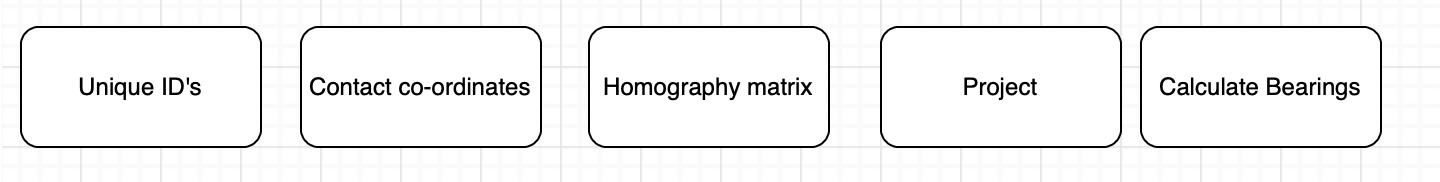
\includegraphics[width=1.0\columnwidth]{temp.png} 
\end{tabular}
\captionof{figure}{Data pipeline overview} 
\label{pipeline}

\subsection{Data Collection}

The Yrsas Plads junction in Copenhagen was chosen as the location for our primary data collection. 
This junction faces several challanges producing “conflicts, unsafe situations, illegal road user behaviour and great dissatisfaction among road users at the intersection” \cite{CPHpost_2021}.
These challenges make the Yrsas Plads junction one of the more complicated junctions in Copenhagen and would serve as a good base to this quantitative analysis method. 
As this is a large junction we have implmented a two cameras recording setup on opposite side of the junction, this provides good coverage regardless of traffic obstructions.

\subsubsection{Recording Location}

There are three consideration to take into account when applying these methods to a junction.
\begin{itemize}
	\item Junction size
\end{itemize}
Larger junctions would require a two camera setup as detailed, but this might not be optimal for intersections much Larger
than the Yrsas Plads junction. A larger junction might require more cameras which will need some implmentation tweeks.
\begin{itemize}
	\item Camera mounting points
\end{itemize}
\begin{itemize}
	\item Junction composition
\end{itemize}

\subsubsection{Camera Selection}

Modern mobile phones offer high resolution and quality cameras in a compact design. We used an LG G6 and a Samsung S7 Edge for recording the junction.
These devices offer wide enough field-of-views (FOV) to record the parts of the junction we are interested in from the selected mounting locations.
FOV being the maximum area a camera can image. A formal method of selecting a recording device would be to select one that has a large enough FOV that can image the entire junction 
from the mounting position that is closest to the junction. Given a recording location we can calculate the FOV needed using equation \ref{eq:1}.
If $\theta > FOV$ then the FOV is too small. Label image.

\begin{equation}
    \theta = tan^-1(\frac{\frac{width}{2}}{adjacent}) * 2\label{eq:1}
  \end{equation}

\ \\ 
  \begin{figure}[h]
    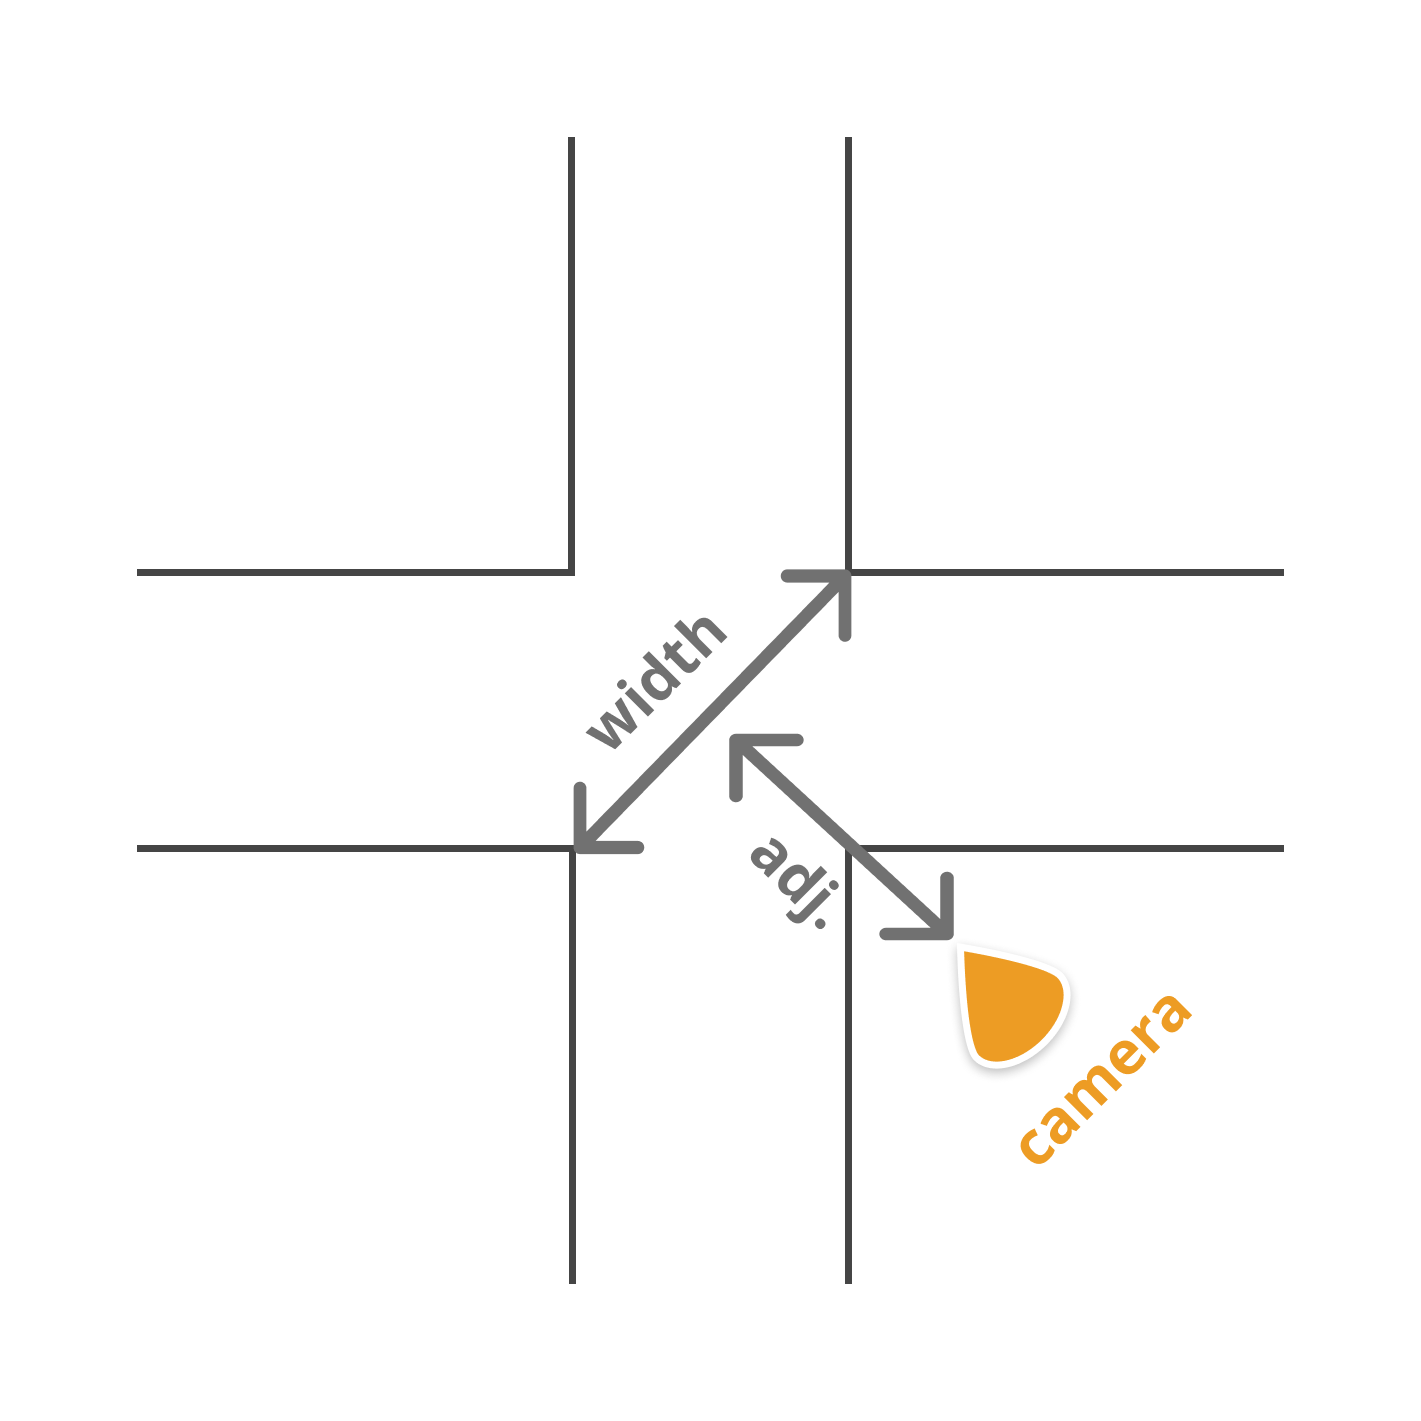
\includegraphics[scale=1.0]{location.png}
    \centering 
    \end{figure}
    \captionof{figure}{Barrel Distortion}
    \label{Camera location}

Battery life and storage capacity should also being considered depending on the amount of intended recording. 
With regards to storage a good estimate for video size would be 149MB per 1 min of FullHD (1920*1080) at 30FPS, storage should be selected
with the intended amount of recording time.

\subsection{Data Processing}

\ \\ 
\noindent
\begin{tabular}{@{}cc}
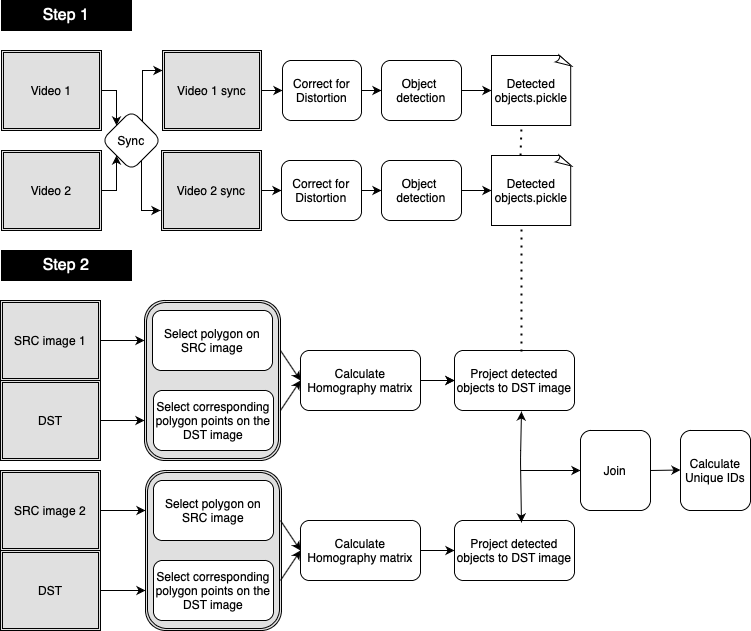
\includegraphics[width=1.0\columnwidth]{data_flow.png} 
\end{tabular}
\captionof{figure}{Data Pipeline}
\label{data}


Figure \ref{data} offers a general overview of the data processing steps. No special hardware is required, but a CUDA enabled GPU
device would be optimal for object detection.
\ \\
\subsubsection{Distortion Correction}

Cameras often suffer from optical aberration where straight lines appear bent. This is specifically observable on 
wide angle camera lenses such as that on the LG G6 used in this study.
The specific type being positive radial distortion such as in figure \ref{distortion}, where lines curve outwards in a shape of a barrel.
Another form of radial distortion is pincushion distortion where lines bend towards the centre of the image. These aberrations are a result 
of the curved shape of the camera lens.

\ \\ 
\begin{figure}[h]
  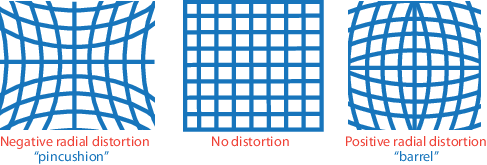
\includegraphics[scale=0.65]{calibration_radial_distortion.png}
  \centering 
  \end{figure}
  \captionof{figure}{Distortion}
  \label{distortion}

\ \\

There is also a possability of further distortion if the camera sensor and the lense are not parralel, this is known as tangential distortion.
Ideally, there should be no radial nor tangential distortion.
\ \\
Distortion can lead to incorrect projection and therefore joining of video sources later on.
To correct for this we make use of OpenCVs \cite{noauthor_opencv/opencv_2021} camera calibration toolbox.

In order to correct for distortion we need to find the camera matrix and distortion coefficients... Explain the maths a bit more.
\ \\
\subsubsection{Object Detection}

The raw video is output as a .mp4 file this video file is if fed to YOLO v5 for object detection. YOLO, You Only Look Once,
is a real-time object detection algorithm. YOLOv5 is trained on the COCO dataset \url{https://cocodataset.org}, which comprises over 330,000 thousand images
with over 1,5 million objects in over 80 object classes.
\ \\ 
YOLO is well known for its real-time speed and accuracy \cite{redmon2016look}.
\ \\ 
At the most basic level YOLO resizes an input image, runs a single convolutional network on the resized image
and then thresholds the resulting detections by the model’s confidence.
\ \\ 
Predicted objects are represented as bounding boxes with output being represented as in \ref{representation} 

\begin{equation}
  [ [frame id][xmin][ymin][xmax][ymax][confidence]]\label{representation}
\end{equation}

The min and max values for x and y represent a bounding box for the identified bicylce.

\subsubsection{Homography Matrix}

An homography matrix is a transformation matrix between two planes \cite{hartley_zisserman_2004}. It can be used to perform a perspective transformation of a plane from a source image $P(x_r, y_r)$ onto a plane on a destination image $Q(x_i, y_i)$.
The source image in our case being the plane of the road surface from the recorded video at the intersection to the road surface from an aerial view of the same intersection.  
This will allow us to view the cyclist movements from an aerial view.
\ \\ 
\begin{figure}[h]
  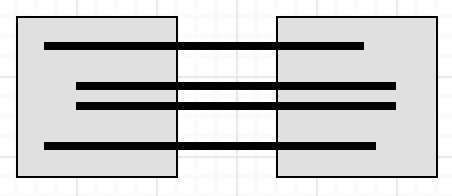
\includegraphics[scale=1.0]{Homography_proj.png}
  \centering 
  \end{figure}
  \captionof{figure}{SR to DST}
  \label{homography}
\ \\ 
To calculate the homography matrix we need to solve the for the system of linear equations \ref{eq:2}

\begin{equation}
  P = HQ\label{eq:2}
\end{equation} 

Referencing \ref{eq:3}, $P$ being points in a polygon on the source image, $Q$ the corresponding polygon on the destination image $H$ being the homography matrix.
\begin{align}
\label{eq:3}
  \begin{bmatrix}
    x_{i} \\
    y_{i} \\
    z_{i} \\
  \end{bmatrix}
  &= \begin{bmatrix}
      h_1 & h_2 & h_3 \\
      h_4 & h_5 & h_6 \\
      h_7 & h_8 & h_9 \\
  \end{bmatrix}
  \begin{bmatrix}
    x_{r} \\
    y_{r} \\
    z_{r} \\
  \end{bmatrix}
\end{align}

\subsubsection{Projection}

Before we can project the cyclist onto an aerial view we first need to calculate teh $(x, y)$ coordinates of their contact points with the road surafce.
Given \ref{representation} we can calculate this by \ref{eq:4}

\begin{align}
  x = xmin + \frac{(xmax - xmin)}{2} 
  y = ymin\label{eq:4}
\end{align} 

Using the homography matrix we can now project the contact points $(x, y)$ of the cyclist onto the destination
image. This is achieved by applying $z$ to each point as a constant so as to create $Q(x_i, y_i, 1)$ and then we multipy it by 
homography matrix. 

\subsubsection{Merging Sources}

To merge the data from the two video sources we take a naive approach. For optimal coverage the cameras are setup on
opposite sides of the junction. To join them we simply cut the video sources in half along the halfway point between
the two cameras along the junction. The data is then merged.

\subsubsection{Multiple object tracking}

In order to connect observations into trajectories of individual cyclist we apply 
simple online and real time tracking algorithm, SORT \cite{abewley_abewley/sort_2021}, as initially described in \cite{Bewley2016_sort}. 
SORT aims to address the problem of multiple object tracking (MOT) where object across frames needs to be connected. 
Note: Explain more about SORT predict bbox then iou for actualy bbox.
\ \\
To join the tracks from multiple sources we assume arbitrary bounding box dimensions of 10*10 pixels for the projected cyclists. 
Passing the algorithm the bounding boxes per frame we get a unique ID associated with each observation.

\subsection{Data Exploration}

There are two objectives for the data exploration, those being:
\begin{itemize}
	\item Desire path discovery
	\item Alert Zones - For behaviour observations and counts
\end{itemize}

\subsubsection{Rainbow Tracks}

A method of Desire path discovery.

\ \\ 
\noindent
\begin{tabular}{@{}cc}
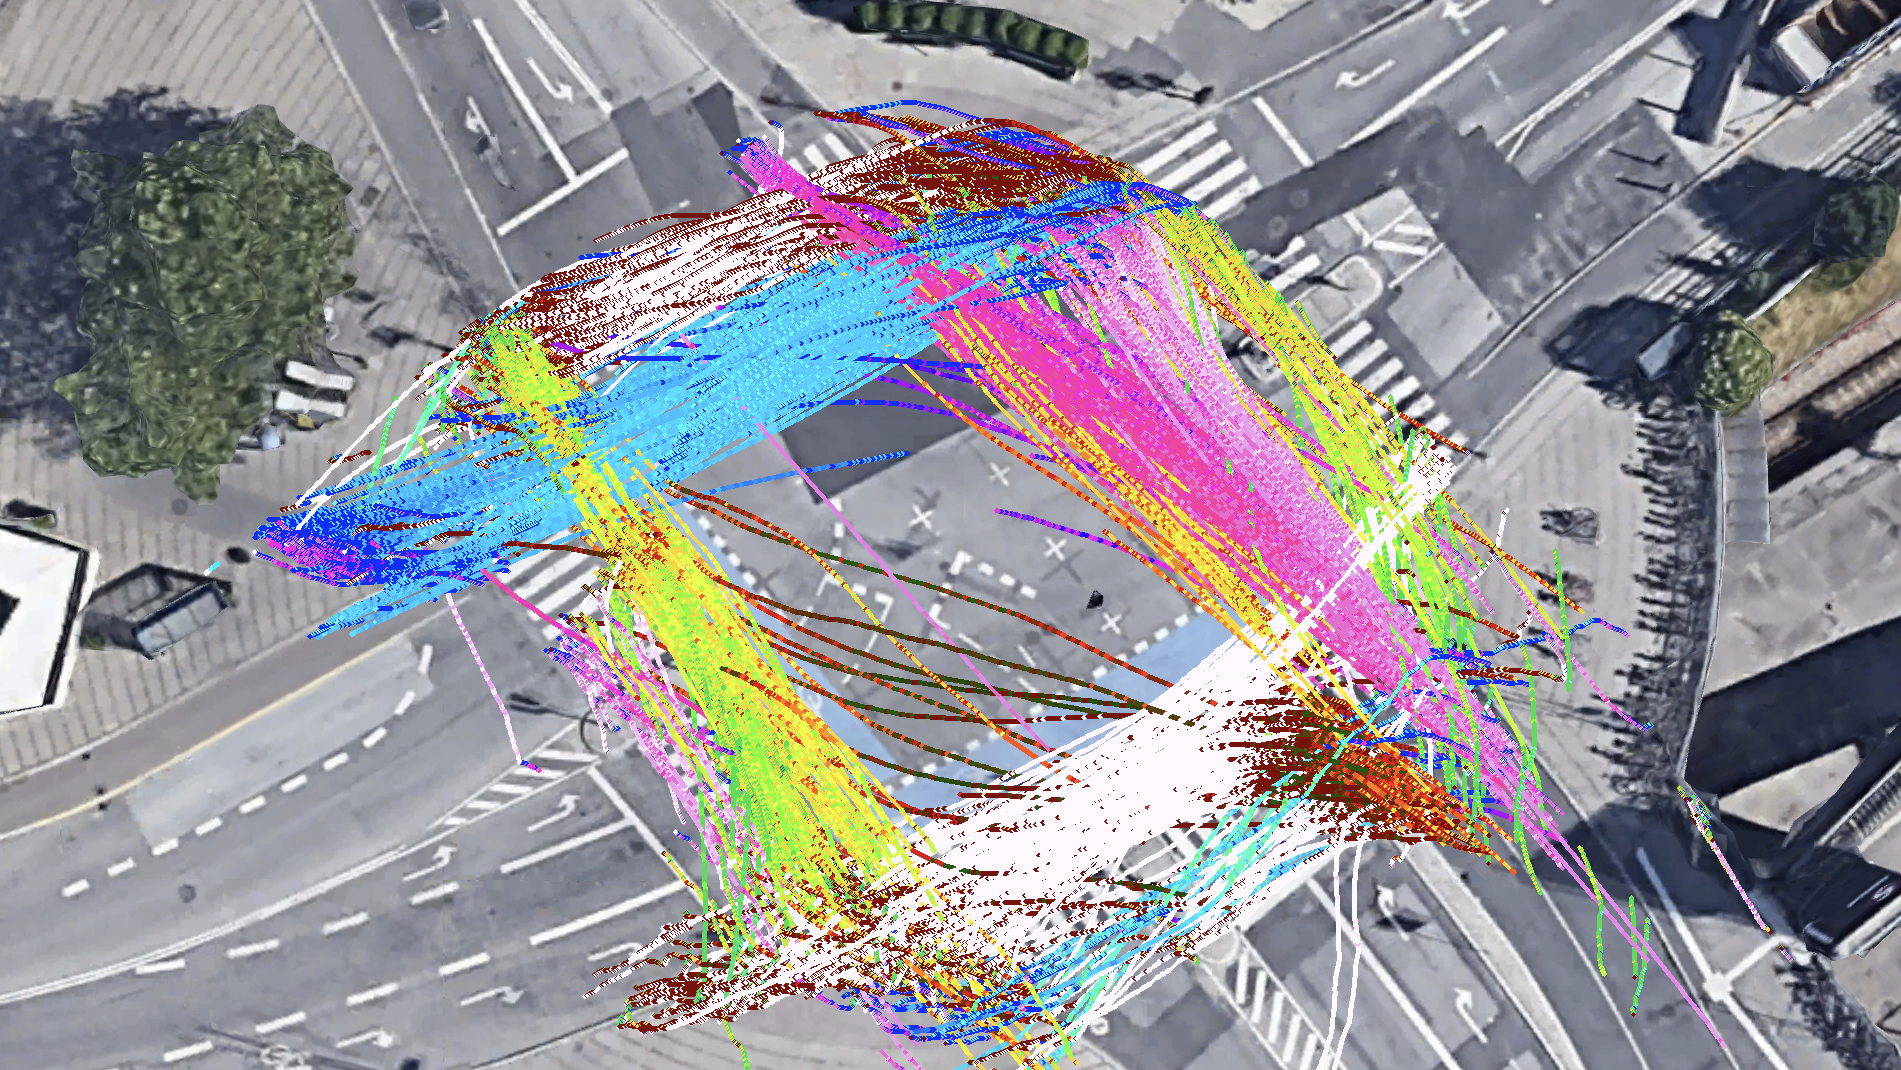
\includegraphics[width=1.0\columnwidth]{rainbow.png} 
\end{tabular}
\captionof{figure}{Rainbow}
\label{Rainbow}

To find aggregated desire lines from the data we took an approach which we call "Rainbow tracks". This involves coloring tracks by the bearing between consequtive points in each 
trajectory, after calculating the bearing we then get a color from a gardient color wheel. This approach has the added benefit of encoding direction into 
each track.
Note: Maybe just an equation demonstaring the bearing calculation.
\ \\ 
\begin{equation}
  UniqueID_i = [(x_1, y_1)...(x_a+1, y_a+1)]\label{eq:3}
\end{equation}

\subsubsection{Alert Zones and Counts}

We created a "Tool name", that allows the defining of certain areas as "Red zones". These zones are provide us with easy reference to activty in the zones throught the videos.
Using these zones we can count cyclist and observe their behaviour at points on the junction that might be difficult or
problematic.

Note: Picture of interface?
